\chapter{Experiment}

In the Experiment an Austrian one cent coin was examined. The goal of the experiment is to understand the principle of the OCT and get to know the usage of the system.

\section{Start-up of the OCT system}

To start the OCT-system first the measurement computer, the scanning mirror drivers, the detector unit and the Laser has to be switched on. The laser is operational if the LED labled 'ready' is on. At the measurement computer the LabView program 'OCT\_student.vi' is started.

To check the functionality of the system a 'continuous scan' is performed. The current plots of the A-scan in k-space and z-space are shown in the LabView window. In the A-scan in z-space a peak is visible. This represents the position of the surface of the sample. The position of the sample can be moved by a positioning screw. If the position of the peak is moved below zero, another peak becomes visible moving in positive direction. Thus the modulation of the A-scan in k-space consists of two symmetrical peaks in z-space. Since k-space and z-space are related by a Fourier transform (cf. \ref{sec:fourier}), the modulation carrying the information must be sinusoidal. \comseb{versteht man das?}
With this setup only the difference of the optical path length of the reference and the sample arm is measured. So when moving the peak below zero, another peak becomes visible moving in positive direction. 
\comwo{ist es nicht so?}
When turning on the positioning screw and moving the sample, the amplitude of the peak in z-space changes. This is because of the lens that focuses the beam on the sample. The maximum peak amplitude is when the beam is focused. By moving the sample out of the focus the amplitude gets smaller.

As another check, the optical path was one time blocked at the sample side and one time at the reference side. If this is done, in both ways the peak in z-domain vanishes, because there is no more interference. Though the A-scans in z-domain differ significantly. 
If the reference path is blocked, only the back scattered light of the sample hits the detector. Thus the intensity of the detected signal is orders of magnitude higher in the case of a blocked sample path.


\section{Performing a 3D-scan of the sample}

In the next step a 3D scan of an Austrian one cent coin was recorded. The sample was mounted in the OCT-System by the advisor of the experiment in advance. Then the range of scanning is set by the rotation angle and the stepsize in x- and y-direction. The obtained measurement data is now analyzed by the MATLAB script 'OKT\_OCT\_3D.m'. 

At first the variables of the script needed to be defined. Therefore the in LabView chosen settings as angle and the number of steps in x- and y- direction were inserted.\comseb{das w�rde ich eigentl weglassen}

By setting the parameters \textsc{zmin} and \textsc{zmax} the region of interest can be defined in meters.

For each A-scan the z-position of the peak is detected. This is done by finding the maximum of the reflectivity in z-domain. The obtained values are writen into a matrix at the corresponding (x,y)-position.

At the last the data is displayed in four surface plots. In the first plot, all A-scans in k-space are shown. In the second and third plot all A-scans in z-space are shown. In the third plot, only the range defined by \textsc{zmin} and \textsc{zmax} is displayed. Lastly in the fourth plot the Matrix calculated earlyer is displayed. It shows the 3 dimensional surface of the sample.

The scan was first performed with an angle between -10� to 1� in x-direction and an angle of -7� to 7� in y-direction. The step size was chosen as 1� for a first try. The resolution of the obtained 3D-surface was very low, so a lower stepsize had to be chosen. When trying a stepsize of 0.1� the LabView interface crashed. This becomes clear when the amount of data is considered. Each A-scan contains of $n_{A-scan}=$1536 measured values in k-space.






\begin{figure}%
\centering
%\begin{adjustwidth}{0cm}{0cm}
	\subfloat[Measured profile]{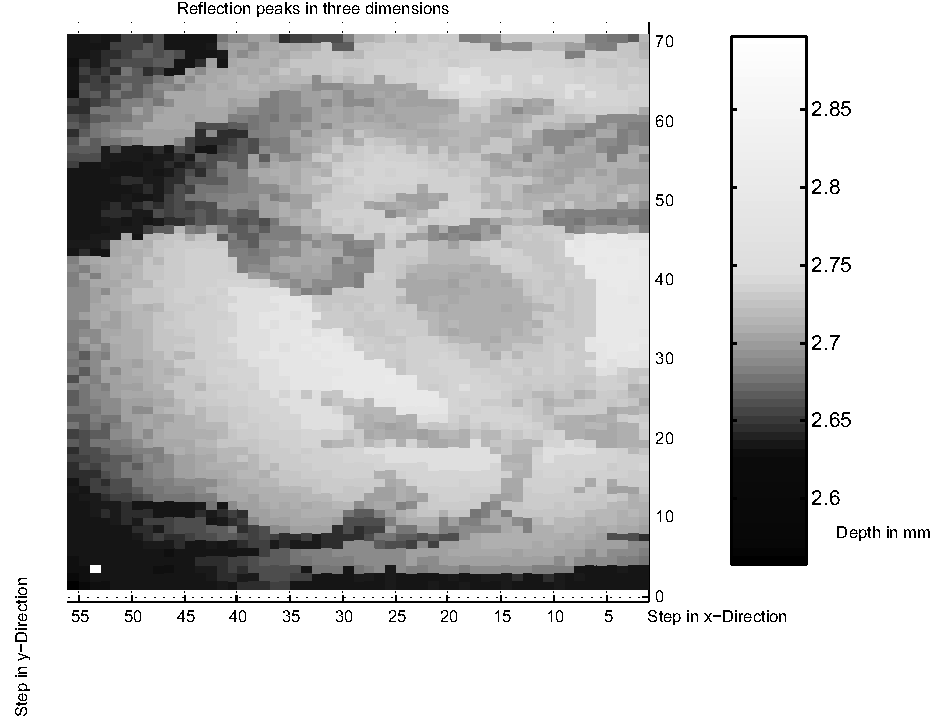
\includegraphics[totalheight=6 cm]{Grafiken/3d_0_2.pdf}\label{fig:Profil_3D}~}
	\subfloat[Austrian 1 ct. coin]{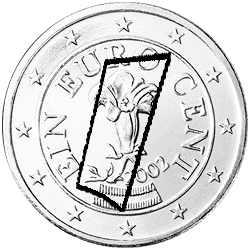
\includegraphics[totalheight=6 cm]{Grafiken/1ct.jpg} \label{fig:1ct}}%
%\end{adjustwidth}
\caption{\textbf{a)} Measured profile of a coin with a stepsice of 0.2�.  \textbf{b)} Austrian 1 ct. coin.}%
\label{fig:Coin}%
\end{figure}

Figure \ref{fig:Profil_3D} shows the result of the measurement with a stepsice of 0.2�. The depth of the surfaces is color-coded.  For comparison figure \ref{fig:1ct} shows a Austrian 1 cent coin\footnote[1]{Source: European Central Bank} with the section marked that is shown in \ref{fig:Profil_3D}.